\documentclass{article}

% if you need to pass options to natbib, use, e.g.:
%     \PassOptionsToPackage{numbers, compress}{natbib}
% before loading neurips_2020

% ready for submission
% \usepackage{neurips_2020}

% to compile a preprint version, e.g., for submission to arXiv, add add the
% [preprint] option:
%     \usepackage[preprint]{neurips_2020}

% to compile a camera-ready version, add the [final] option, e.g.:
%     \usepackage[final]{neurips_2020}

% to avoid loading the natbib package, add option nonatbib:
\usepackage[nonatbib]{neurips_2020}
\usepackage[utf8]{inputenc} % allow utf-8 input
\usepackage[T1]{fontenc}    % use 8-bit T1 fonts
\usepackage{hyperref}       % hyperlinks
\usepackage{url}            % simple URL typesetting
\usepackage{booktabs}       % professional-quality tables
\usepackage{amsfonts}       % blackboard math symbols
\usepackage{nicefrac}       % compact symbols for 1/2, etc.
\usepackage{microtype}      % microtypography
\usepackage{amsmath}
\usepackage{amssymb}
\usepackage{geometry}
\usepackage{float}%稳定图片位置
\usepackage{graphicx}%画图
\usepackage{wrapfig}
\usepackage{indentfirst}%缩进
\usepackage{enumerate}%加序号
\usepackage{multirow}%合并行
\usepackage{subfigure}
\usepackage[bottom]{footmisc}
\usepackage{listings}
\usepackage{xcolor}




\title{VE485 Final Report   }
\author{Chongdan Pan 
\\\texttt{panddddda@sjtu.edu.cn}
\\516370910121 
}
\begin{document}
\maketitle
\begin{abstract}
    This article gives an introduction on a famous generalized linear supervised learning classifier called Support Vector Machine, as known as SVM. SVM was developed in decades ago, and has already been used in various fields ranging from image recognition to data analysis. For linear SVM, it uses hard margin or soft margin with Lagrangian dual to find the optimized hyperplane for classification. For nonlinear SVM, its uses the kernel tricks to project the data into another dimension for classification. This article also discussed the frontiers of SVM and proposed a supervised learning problem to solve through SVM with kernel trick, which is to classify two interlocked ring based on a small fraction of training set. Besides, since the kernel trick can also be applied to unsupervised learning model such kernel PCA, this article will also discuss KPCA's performance to solve this problem without label.
\end{abstract}
\section{Background}
SVM is a supervised learning model, which means it needs to learn from classified data with labels. Given a set of training examples, each marked as belonging to one or the other of two categories, an SVM training algorithm builds a model that assigns new examples to one category or the other\cite{1}.
\section{Linear SVM} 
\subsection{Hard Margin}
SVM was first developed by Vladimir Vapnik and Alexey Chervonenkis in 1963, as a simple linear classifier. Consider a simple case, where we want to classify objects into to categories. We'll use $x\in\mathbb{R^n}$ to describe its features and $y\in{-1,1}$ to describe the result of classification, where -1 and 1 each represents one category\cite{2}.
\par Given training data $(x_1,y_1)\cdots(x_N,y_N)$, The model will try to generate a hyperplane such that the new examples can be assigned to two sides of it, which are corresponding two categories. Any hyperplane can be defined as $w^Tx-b=0$, where $w$ is the normal vector of the hyperplane, defining its direction, and $b$ is the offset.
\par Since the hyperplane is linear, SVM is a binary linear classifier by giving a concrete rather than giving the probability. If the training data is linearly separable, we can select two parallel hyperplanes that separate the two classes of data, so that the distance between them is as large as possible. We can define the two parallel hyperplanes as:
\begin{center}
    $w^Tx-b=1$ where $w^Tx_i-b\geq1\forall y_i=1$
    \\$w^Tx-b\leq-1$ where $w^Tx_i-b\leq-1\forall y_i=-1$
\end{center}
Then for any hyperplane for separation, we can define it as:
$$y_i(w^Tx-b)\geq1,\forall i$$
The region bounded by these two hyperplanes is called the "margin", and the data on these two hyperplanes are called support vectors because they control the margin as well as the hyperplanes. The margin is:
$$\frac{2}{||w||_2^2}$$
The best hyperplane for separation is the maximum-margin hyperplane with largest margin. It is best because when we add the new data, the maximum-margin hyperplane reduces the generalization error the most. So the classification can is an optimization problem:
$$\min_{w,b}\quad \frac{||w||^2_2}{2}$$
s.t.
$$y_i(w^Tx_i-b)\geq1,\forall i$$
    \begin{figure}[H]
        \centering
        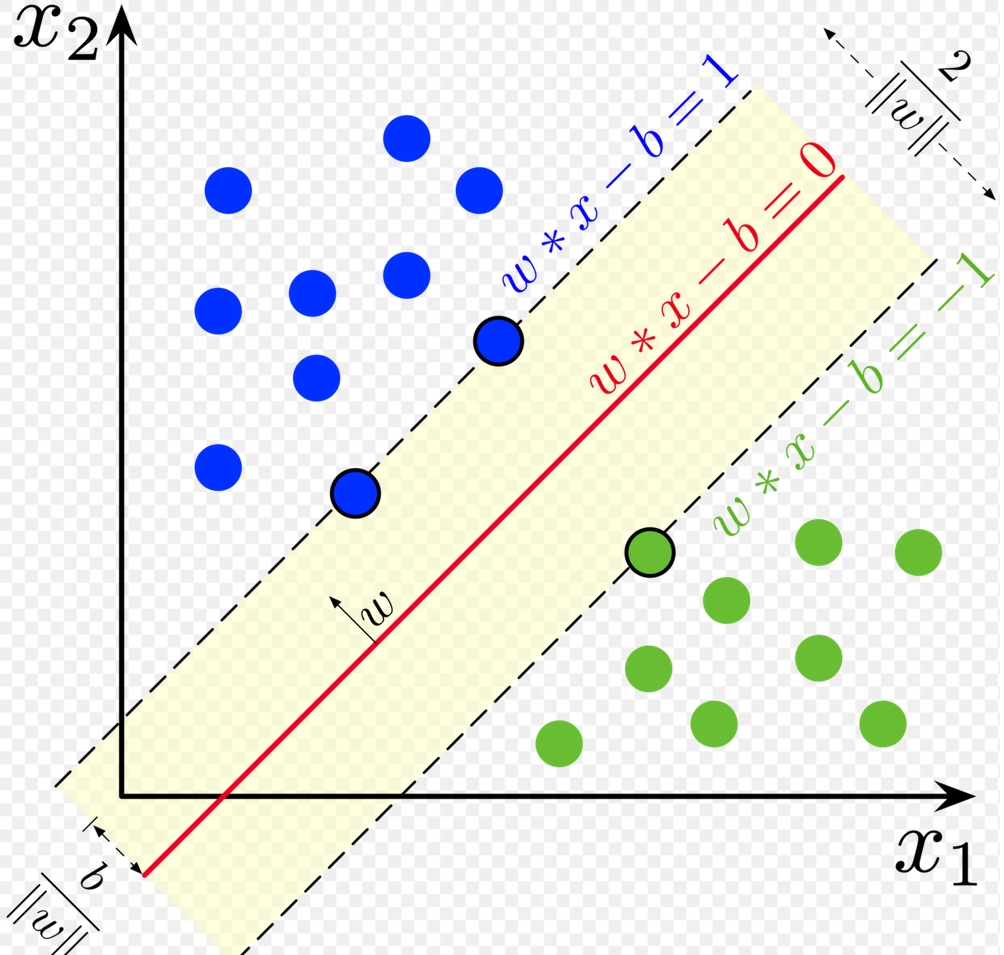
\includegraphics[scale=0.25]{P1.jpg}
        \caption{hyperplanes for classification}
    \end{figure}
\paragraph{Solution}
We can convert it into a Lagrangian Dual problem with $\alpha_i$ as the Lagrangian multiplier, the original problem is equal to: 
$$\min_{w,b}\max_\alpha\mathcal{L}(w,b,\alpha_i)=\frac{||w||^2_2}{2}+\sum_{i=1}^N\alpha_i[1-y_i(w^Tx_i-b)]$$
s.t.
$$\alpha_i\geq0,\forall i$$
We can calculate the minimization first:
$$\frac{\partial\mathcal{L}}{\partial w}=0\Rightarrow w=\sum_{i=1}^N\alpha_iy_ix_i$$
$$\frac{\partial\mathcal{L}}{\partial b}=0\Rightarrow \sum_{i=1}^N\alpha_iy_i=0$$
Plug the result back, our problem becomes: 
    $$\max_\alpha\quad\sum_{i=1}^N\alpha_i-\frac{1}{2}(\sum_{i=1}^N\alpha_iy_ix_i)^2$$
s.t.
    $$\sum_{i=1}^N\alpha_iy_i=0$$
    $$\alpha_i\geq0$$
\begin{itemize}
    \item When $\alpha_i=0,w=0$ and every point is classified in the right category.
    \item When $0<\alpha_i$ according to KKT condition, $0<\alpha$ only when $y_i(w^Tx_i-b)=1$ ,so the hyperplane depends on data on the boundary of right category
\end{itemize}
The hyperplane can be defined as $w^Tx-b,$ where $w=\sum_{i=1}^N\alpha_iy_ix_i,b=w^Tx_i-y_i,$ and $i$ is only for data on the boundary.
\subsection{Soft Margin}In 1995, Corinna Cortes and Vapnik proposed the idea of soft margin by using \emph{hinge loss function} in the process of training. Assume current maximum-margin hyperplane is defined as $w^Tx_i-b=0$. Then the corresponding hinge loss function is defined as:
$$L(x_i)=\max(0,1-y_i(w^Tx_i-b))$$
If the $i_{th}$ training data is classified in the right category by the hyperplane $w^Tx_i-b=0$, then $w^Tx_i-b\geq1$ when $y_i=1$ or $w^Tx_i-b\leq-1$ when $y_i=-1$. Hence, $1-y_i(w^Tx_i-b)\leq0$ and $L(x_i)=0$. If the data is misclassified in the wrong category, then $L(x_i)>0$ and its value increase with the distance between $x_i$ and the hyperplane. The blue line in figure.\ref{hl} shows the graph of \emph{hinge loss function}.
\begin{figure}[H]
    \centering
    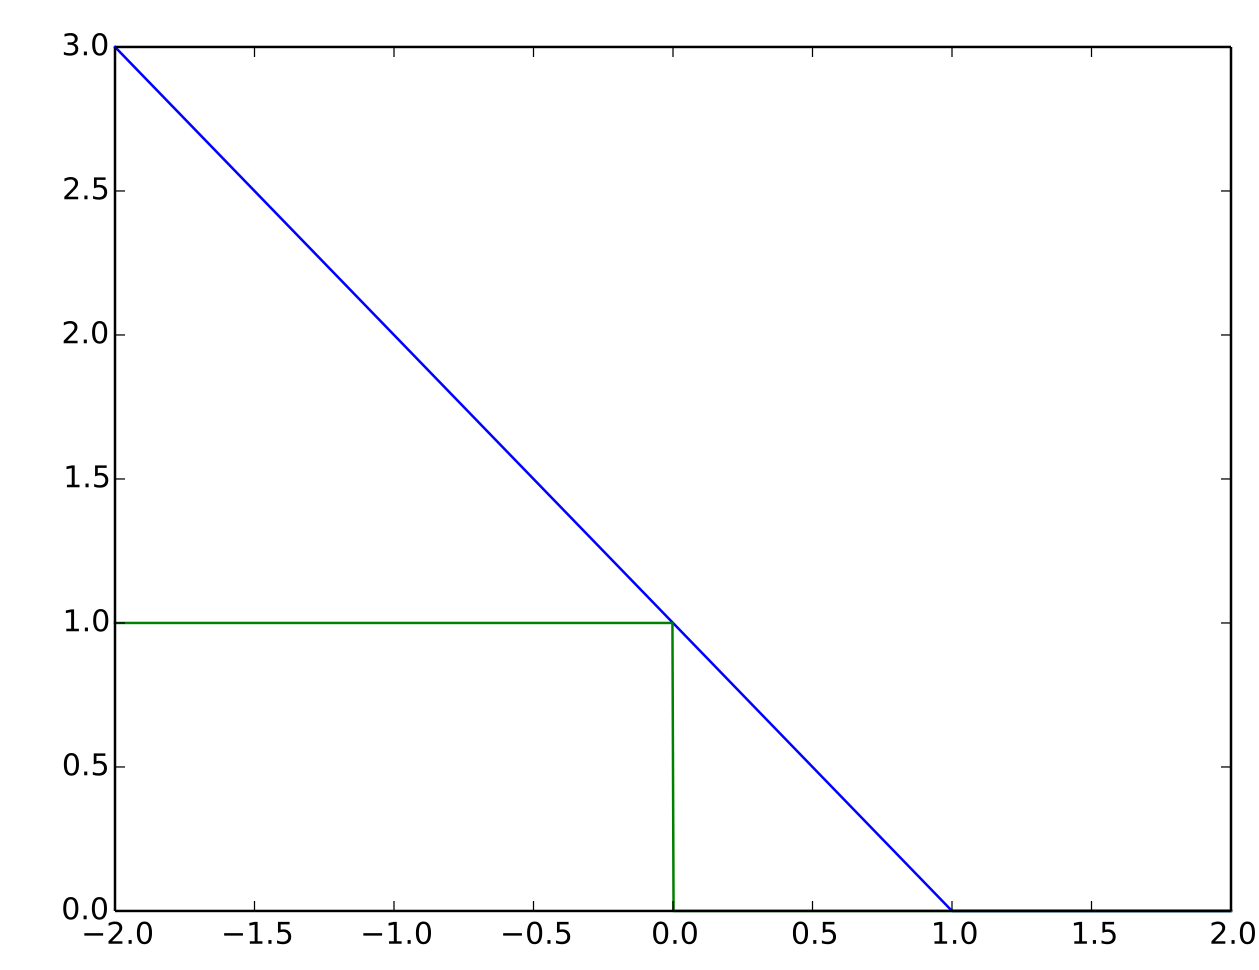
\includegraphics[scale=0.2]{P2.jpg}
    \caption{Loss Function}
    \label{hl}
\end{figure}
\emph{Hinge loss function} only focus on the training data misclassified in the wrong category. Compared to the green line, which is the zero-one loss function, \emph{hinge loss function}'s value shows that how wrong the misclassification is. Then our optimization problem becomes:
$$\min_{w,b} C\sum_{i=1}^NL(x_i)+\frac{1}{2}||w||_2^2$$
The first part is to minimize the distance between wrongly classified data and its correct category, while the later part is the regularization term to minimize the complexity of the linear plane. 
\par For linear separable data set, the soft margin can't necessarily achieve the right classification result as hard margin because it may omit some outliers, but it can have a better result when generalized. For linear inseparable data, although the maximum-margin hyperplane generate from hinge loss function can't necessarily ensure all data in the right category, which is impossible in its dimension, it still can have the relative best classification result, where the misclassified data are close to their correct category as much as possible.
\paragraph{Solution}
Let $\zeta_i=L(x_i)$, then the problem can be rewritten as 
$$\min_{w,\zeta,b}\quad C\sum_{i=1}^N\zeta_i+\frac{1}{2}||w||_2^2$$
s.t.
$$-\zeta_i\leq0,\forall i$$
$$1-\zeta_i-y_i(w^Tx_i-b)\leq0,\forall i$$
We can convert it into a Lagrangian Dual problem with $\alpha_i,\beta_i$ as the Lagrangian multiplier:
$$\mathcal{L}(w,\zeta,b,\alpha,\beta)=\frac{1}{2}||w||_2^2+C\sum_{i=1}^N\zeta_i+\sum_{i=1}^N\alpha_i(1-\zeta_i-y_i(w^Tx_i-b))-\sum_{i=1}^N\beta_i\zeta_i$$
The original problem is equal to: 
$$\min_{w,\zeta,b}\max_{\alpha,\beta}\mathcal{L}(w,\zeta,b,\alpha,\beta)$$
s.t. 
$$\alpha_i\geq0,\forall i$$
$$\beta_i\geq0,\forall i$$
We can calculate the minimization first:
$$\frac{\partial\mathcal{L}}{\partial w}=0\Rightarrow w=\sum_{i=1}^N\alpha_iy_ix_i$$
$$\frac{\partial\mathcal{L}}{\partial b}=0\Rightarrow \sum_{i=1}^N\alpha_iy_i=0$$
$$\frac{\partial\mathcal{L}}{\partial \zeta}=0\Rightarrow \beta_i=C-\alpha_i$$
Plug the result back, our problem becomes: 
    $$\max_\alpha\quad\sum_{i=1}^N\alpha_i-\frac{1}{2}(\sum_{i=1}^N\alpha_iy_ix_i)^2$$
s.t.
    $$\sum_{i=1}^N\alpha_iy_i=0$$
    $$0\leq\alpha_i\leq C$$
\begin{itemize}
    \item When $\alpha_i=0,w=0$ and every point is classified in the right category.
    \item When $\alpha_i=C,\beta_i=0,$ according to KKT condition, $\zeta_i>0$, its value can determine the classification of $i_{th}$ data.
    \item When $0<\alpha_i<C,\beta_i>0,$ according to KKT condition, $0<\alpha$ only when $\zeta_i=0$, so the hyperplane depends on data on the boundary of right category.
\end{itemize}
The hyperplane can be defined as $w^Tx-b,$ where $w=\sum_{i=1}^N\alpha_iy_ix_i,b=w^Tx_i-y_i,$ and $i$ is only for data on the boundary.
\section{Nonlinear SVM}
Actually, in practice, there are scenarios where the data point can't be separated by the linear hyperplane directly in their dimension. For example, Figure.\ref{nlsd} shows data that can't separated by linear hyperplanes.
    \begin{figure}[H]
        \centering
        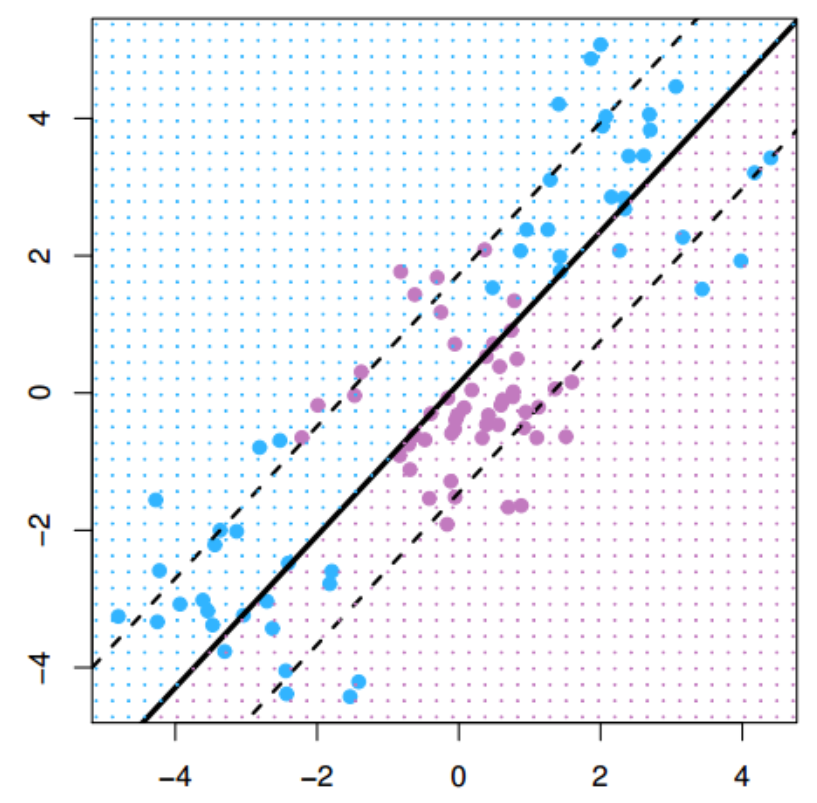
\includegraphics[scale=0.25]{P3.jpg}
        \caption{not linearly separable data}
        \label{nlsd}
    \end{figure}
\subsection{Kernel Method} To solve this question, in 1992, Bernhard E. Boser, Isabelle M. Guyon and Vladimir N. Vapnik suggested a way to create nonlinear classifiers by applying the kernel method to maximum-margin hyperplanes\cite{3}. Kernel method enables SVM operate in a higher or infinite dimension to cope with data in a lower dimension. The hyperplane is still linear in the space with higher dimension, but it's no long linear in the original dimension. 
\begin{figure}[H]
    \centering
    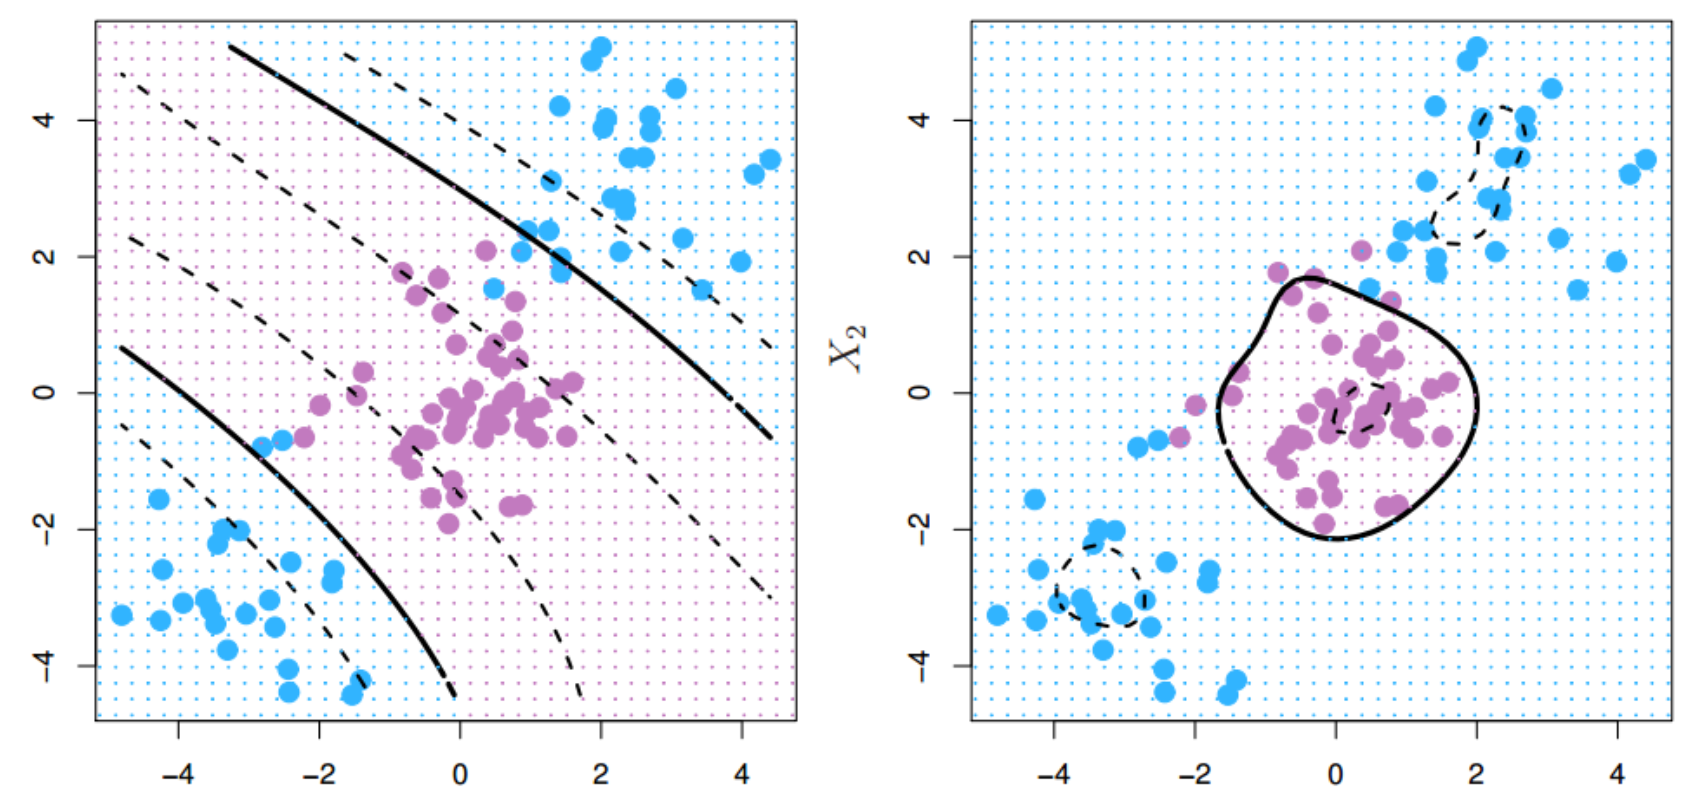
\includegraphics[scale=0.25]{P4.jpg}
    \caption{Data separated non-linearly}
    \label{nlsd}
\end{figure}
To map data from original space to higher dimensional space, SVM first designed a map $\varphi:\mathbb{R}^n\rightarrow\mathbb{R}^{n'},$ and the corresponding kernel function is $\kappa(x_1,x_2)=(\varphi(x_1)^T\varphi(x_2))^2$. Then our original optimization for soft margin is:
$$\max_\alpha\quad\sum_{i=1}^N\alpha_i-\frac{1}{2}(\sum_{i=1}^N\alpha_iy_i\varphi(x_i))^2$$
s.t.
    $$\sum_{i=1}^N\alpha_iy_i=0$$
    $$0\leq\alpha_i\leq C$$
For original support vector hyperplane $w^Tx-b$, where $w=\sum_{i=1}^N\alpha_iy_ix_i$, now it's $\sum_{i=1}^N\alpha_iy_i\kappa(x_i,x)-b$
There are other kinds of kernel functions, but they're all designed to ensure that dot products of pairs of input data vectors may be computed easily in terms of the variables in the original space\cite{4}.
\begin{itemize}
    \item Linear kernel $\kappa(x_1,x_2)=x_1^Tx_2$, the function is very simple, but it's just like there is no kernel function, so it can't treat non linear separable data.
    \item Polynomial kernel $\kappa(x_1,x_2)=(\lambda x_1^Tx_2+\alpha)^\beta$, the function can solve more problems, but it has many parameters and hard to adjust the value.
    \item Gauss kernel $\kappa(x_1,x_2)=\exp(-\frac{||x_1-x_2||^2}{2\gamma^2})$, the function also can solve many problems and it only has one parameter, but it has a high time complexity.
\end{itemize}
\section{Application and Issue}
SVM can be applied in various scenarios, including classifying imagine, text or data and make recognition. It has been developed or used together with other algorithms, such as regression, clustering problems or other tasks like outliers detection. Its idea of kernel function is also being applied in other models. 
\par However, the traditional SVM also has some drawbacks. It must be used in supervised learning, namely requiring full labels of data. It also can only classify samples into two categories. Therefore, multiclass SVM model has been developed for multiple binary classification. Probabilistic SVM also has been developed to output the probability of the example in specific categories, which extend SVM's usage. In addition, the parameters of SVM and kernel function sometimes are difficult to interpret intuitively, hence it's hard for normal users to adjust the model.
\section{Frontiers}
Recent algorithms for finding the SVM classifier include sub-gradient descent and coordinate descent. Both techniques have proven to offer significant advantages over the traditional approach when dealing with large, sparse datasets—sub-gradient methods are especially efficient when there are many training examples, and coordinate descent when the dimension of the feature space is high. 
\subsection{Sub-gradient Descent}
Since our optimization problem wants to find the minimal value of a convex function, a traditional \emph{SGD} can be adapted directly\cite{5}. Instead of taking a step in the direction of the function's gradient, a step is taken in the direction of a vector selected from the function's sub-gradient. For certain implementations, the number of iterations does not scale with the number of data points $N$, hence it can be extremely efficient when there are many training data.
\subsection{Coordinate descent}
The coordinate descent problem are used in the dual problem. The dual coefficient $\alpha_i$ is adjusted in the direction of $\frac{\partial\mathcal{L}}{\partial \alpha_i}.$ The the result $c_i'$ is projected onto the nearest vector of coefficients that satisfies the given constraints. The resulting algorithm is extremely fast in practice, although few performance guarantees have been proven\cite{6}.
\subsection{Multiclass SVM}
Multiclass SVM aims to assign labels to instances by using support-vector machines, where the labels are drawn from a finite set of several elements. The dominant approach for doing so is to reduce the single multiclass problem into multiple binary classification problems\cite{7}. 
\subsection{Support Vector Clustering}
Support Vector Clustering is called SVC in short. It was created by Hava Siegelmann and Vladimir Vapnik, applies the statistics of support vectors, developed in the support vector machines algorithm, to categorize unlabeled data. It has a similar principle to kernel cluster by finding a ball in the higher dimension space generated by the kernel function\cite{8}. The ball should encircle all training data with lowest radius. Then the ball will be projected into original space, and each ball is a category. SVC can be used in unsupervised learning and can generate boundaries with any pattern. However, SVC needs to take a lot time in computing the matrix.
\subsection{Regression}
Using SVM for regression was proposed in 1996, which is called support-vector regression (SVR)\cite{9}. The model produced by support-vector classification (as described above) depends only on a subset of the training data, because the cost function for building the model does not care about training points that lie beyond the margin. Analogously, the model produced by SVR depends only on a subset of the training data, because the cost function for building the model ignores any training data close to the model prediction.
\subsection{Bayesian SVM}
In 2011 it was shown by Polson and Scott that the SVM admits a Bayesian interpretation through the technique of data augmentation\cite{10}. In this approach the SVM is viewed as a graphical model where the parameters are connected via probability distributions. This extended view allows the application of Bayesian techniques to SVMs, such as flexible feature modeling, automatic hyperparameter tuning, and predictive uncertainty quantification. Recently, a scalable version of the Bayesian SVM was developed by Florian Wenzel, enabling the application of Bayesian SVMs to big data. Florian Wenzel developed two different versions, a variational inference (VI) scheme for the Bayesian kernel support vector machine and a stochastic version  for the linear Bayesian SVM.
\subsection{Probabilistic SVM}
Probabilistic can be regarded as the combination of logistic regression and SVM. It will calculate the probability through sigmoid function after SVM's classification. The model use zoom and translation parameter $(A,B)$ to make affine transformation on the decision boundary, and use MLE to get (A,B)\cite{11}. The distance between the data and the transformed boundary can be put into sigmoid function and get probability. The optimization is:
$$A,B=\arg\min_{A,B}\frac{1}{N}\sum_{i=1}^N(y_i+1)\log p_i+(1-y_i)\log(1-p_i)$$
$$p_i=\mathrm{sigmoid}[A(w^T\varphi(x)-b)+B]$$
\subsection{Least Square SVM, LS-SVM}
LS-SVM just change the optimization process, where $C\sum_{i=1}^N\zeta_i$ is now changed like $C\sum_{i=1}^N\zeta_i^2$, a form similar to ridge regression\cite{12}. LS-SVM can have a higher efficiency in optimization than normal SVM, and can have same classification result when the training examples are linearly independent.
\section{Problem}
My problem is using the SVM or the kernel trick from SVM to complete a complex classification problem, where the classified data which are coupled together in original dimension. 
\begin{figure}[H]
    \centering
    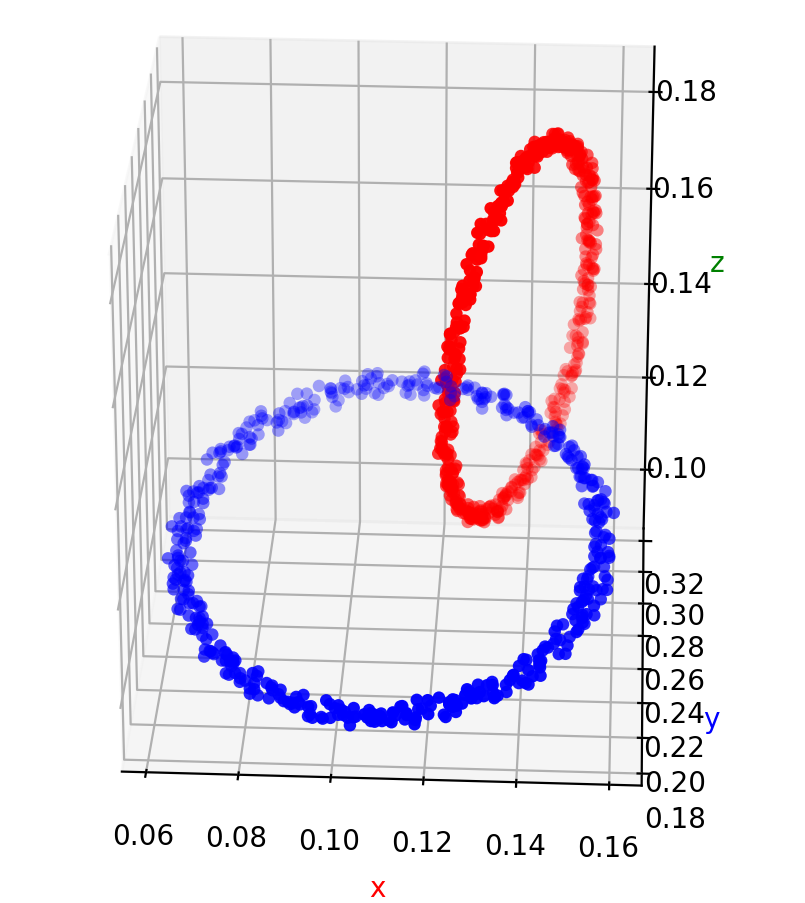
\includegraphics[scale=0.25]{p5.png}
    \caption{An example for the data}
    \label{ring}
\end{figure}
For example, Figure.\ref{ring} shows two rings interlaced in the 3D space, to be classified. Since the data is not linear separable, the significance of this problem lies in the specific selection of kernel function and its parameters. The kernel trick can also be used in the unsupervised learning like kernel PCA. The problem will be set in the following way:
\begin{enumerate}[(a)]
    \item Generate two centers of ring in the $\mathbb{R}^3$ randomly, and the distance between them is 1.
    \item The parameter $r\in[0.5,1]$ ensures the rings are coupled, and we can use $p=(2r-1))/\rightarrow p\in[0,1]$ to donate the ratio of the distance of the edge of two rings over their centers. When $p$ is 1, the edge of each ring pass the other's center, while when $p=0$, two ring's edge are connected together.  The smaller $p$ is, the harder for classification.
    \item After the generation, 500 noise point is added to each ring where its max distance from the ring is $0.2r$
    \item A basis in $\mathbb{R}^3$ is randomly generated to apply linear transformation on original data.
    \item Add label to two circles for SVM training. 10\% of the data is used for training, while the rest 90\% will be used to test.
\end{enumerate}
\section{Solution}
\subsection{Supervised Classification SVM}
I begin with $p=1$, which is the most simple case. It's obvious that the data needs to be transformed into higher dimension for classification, however, the polynomial kernel doesn't perform well even when I set its degree to 25.
\begin{figure}[H]
    \centering
    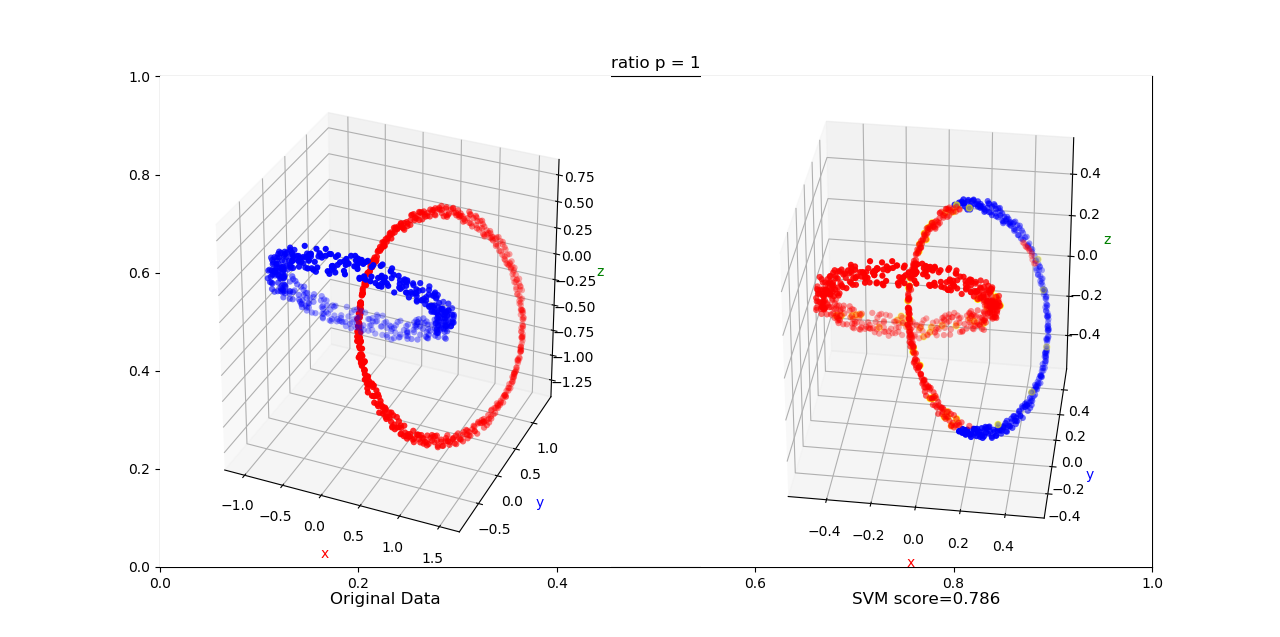
\includegraphics[scale=0.5]{poly.png}
    \caption{Result when polynomial kernel is applied}
    \label{poly}
\end{figure}
From Figure.\ref{poly} we can see that there is a bended plane for classification, however, it is not enough to classify the data. Hence, I will use rbf kernel to classify it in a higher dimension. Recall the form of rbf kernel :
$$\kappa(x_1,x_2)=\phi_{rbf}(x_1)\cdot\phi_{rbf}(x_2)=\exp(-\frac{||x_1-x_2||^2}{2\gamma^2})$$
Assume $x_1,x_2\in\mathbb{R}^2$, then 
$$\kappa(x_1,x_2)=\exp(-\frac{(x_1-x_2)^2+(y_1-y_2)^2}{2\gamma^2})=\exp(\frac{2x_1x_2+2y_1y_2-{x_1}^2-{x_2}^2-{y_1}^2-{y_2}^2}{2\gamma^2})$$
$$\kappa(x_1,x_2)=\exp(\frac{-||x||^2)}{2\gamma^2}\exp(\frac{-||y||^2}{2\gamma^2})\exp(\frac{2x\cdot y}{2\gamma^2})=\exp(\frac{-||x||^2}{2\gamma^2})\exp(\frac{-||y||^2}{2\gamma^2})\sum_{n=0}^\infty \frac{(2x\cdot y)^n}{2\gamma^2n!}$$
$$\phi_{rbf}(x)=\frac{1}{\sqrt{2}\gamma}\exp(\frac{-||x||^2}{2\gamma^2})\sum_{n=0}^\infty(1,\sqrt{\frac{2}{1!}}x,\sqrt{\frac{2^2}{2!}}x^2\cdots,\sqrt{\frac{2^\infty}{\infty!}}x^\infty)$$
Therefore, the rbf kernel can project $x$ from $\mathbb{R}^2$ to $\mathbb{R}^\infty$.
\begin{figure}[H]
    \centering
    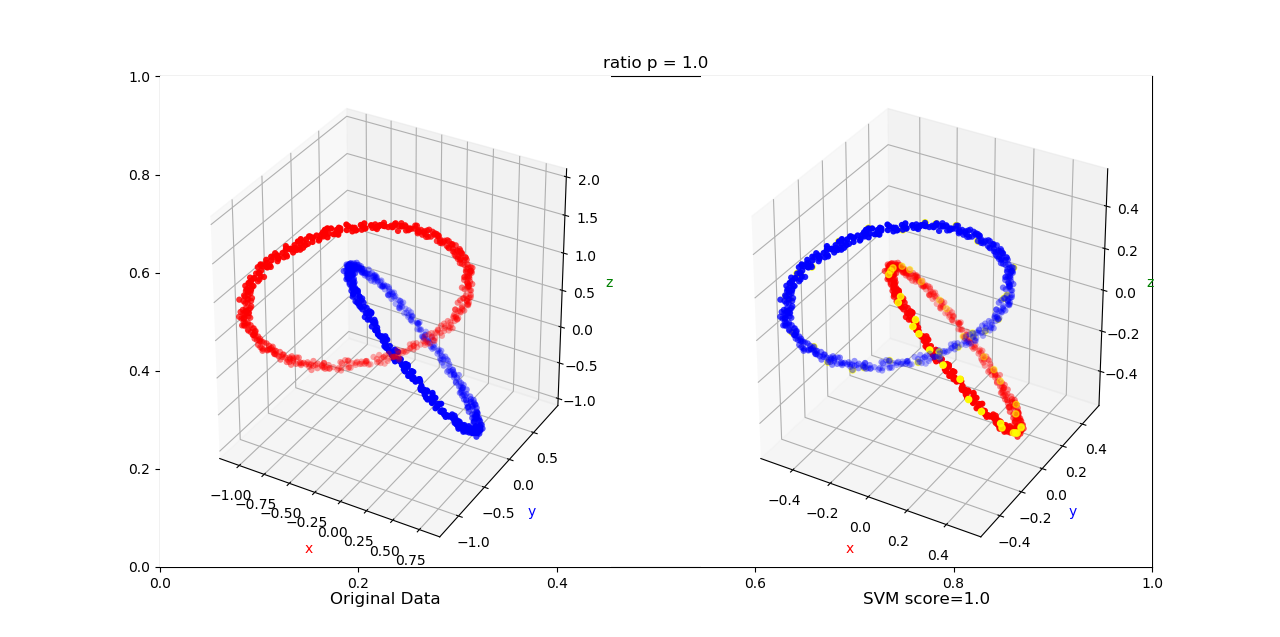
\includegraphics[scale=0.5]{svm.png}
    \caption{Result when $p=1$ and rbf kernel is applied}
    \label{rbf}
\end{figure}
Figure.\ref{rbf} shows that SVM works very well when rbf is applied. The yellow point is the supper vector of the model, and it shows that SVM can achieve great performance even when the training set is not very big as long as the it has enough support vector for classification.
\\However, as we decrease $p$ and make the problem more difficult, the default rbf can't make sure all data is classified well even though it still has a high score.
\begin{figure}[H]
    \centering
    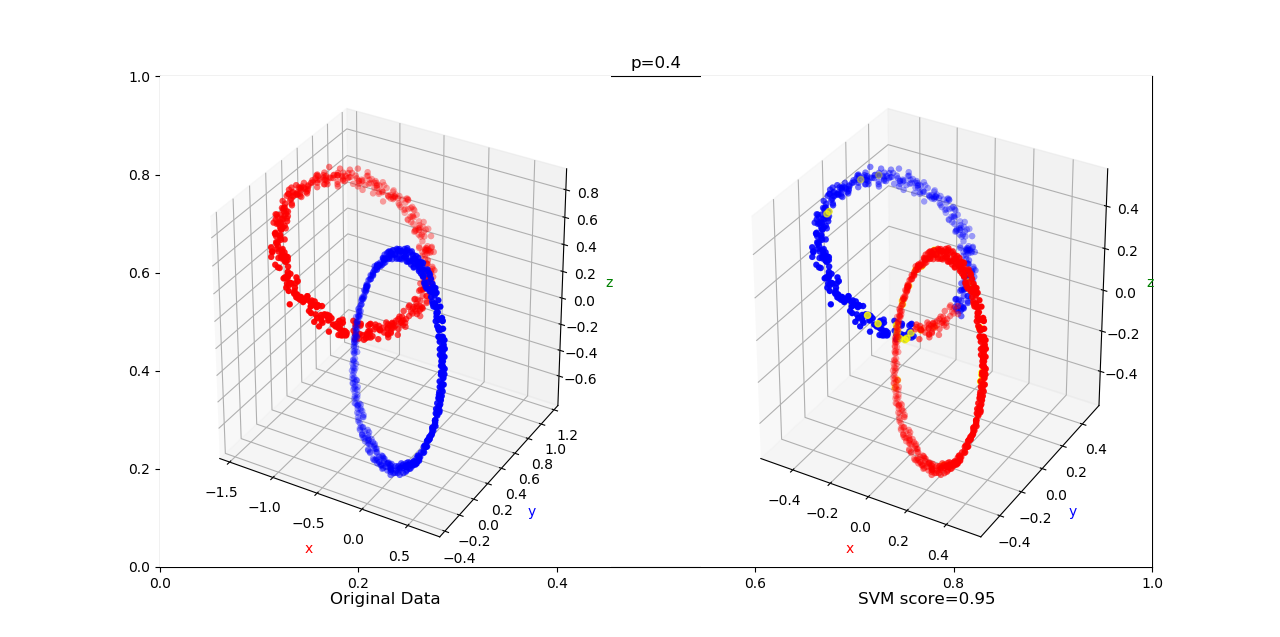
\includegraphics[scale=0.5]{7.png}
    \caption{Result when $p=0.4$ and rbf kernel with $\gamma$=default}
    \label{7}
\end{figure}
Figure.\ref{7} shows that decision boundary can't classify close data points well. 
\begin{figure}[H]
    \centering
    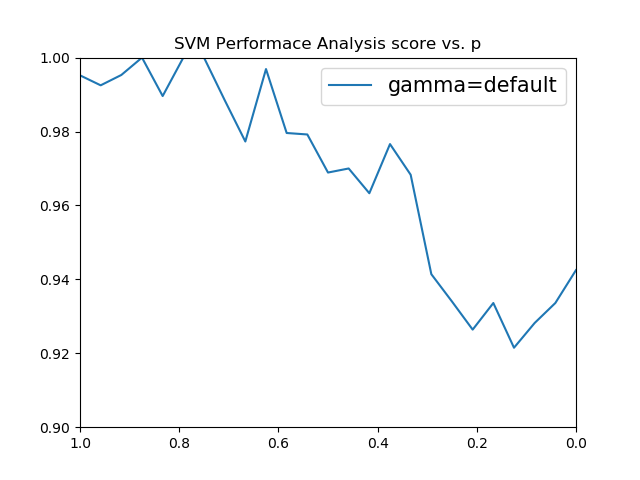
\includegraphics[scale=0.4]{svma1.png}
    \caption{rbf SVM score vs. $p$, $\gamma=$ default}
    \label{svma1}
\end{figure}
I train the model for 5 times at different $p$, and Figure.\ref{svma1} shows that the model's performance get worse as $p$ decreases.
\\To make further improvement, I tune the parameter of the kernel. In essence, a dot product $x_1\cdot x_2$ or a kernel dot product $\kappa(x_1,x_2)=\phi(x_1)\cdot \phi(x_2)$ is measuring the similarity of $\phi(x_1)$ and $\phi(x_2)$ since $\phi(x_1)\cdot \phi(x_2)=|\phi(x_1)||\phi(x_2)|\cos\alpha$. For example, in the rbf kernel, when $x_1=x_2,\kappa(x_1,x_2)=1$, and achieve its maximum value, since $x_1$ and $x_2$ are most similar. Compared to other kernel or original dot product, the result of $\kappa(x_1,x_2)$ only depends on the relative value of $x_1,x_2$. As we increase $\gamma,\kappa(x_1,x_2)$ will increase as well, and it has the same effect as all data points are clustered to the original point.
\\According to Figure.\ref{7}, it seems that there is few support vectors on the misclassified data, which means the model is not sensitive enough to the edge of the data. Therefore, by increasing the value of $\gamma$, we can narrow down the classification radius of each support vector, because if the data points are clustered, the classification area around it will be smaller, however, actually it doesn't. Therefore,
 we will have more support vectors and the classification result will become more splitted like each support vector will have a small classification area. Therefore, the classification result will be more accurate and conformed to the training data.
\begin{figure}[H]
    \centering
    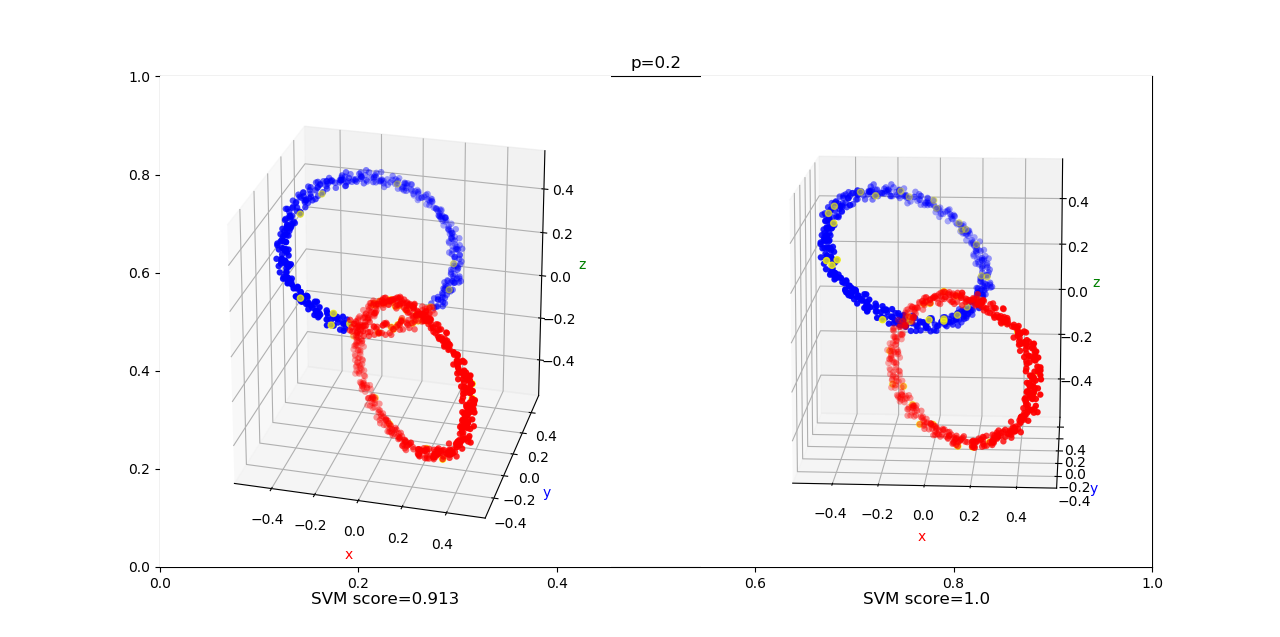
\includegraphics[scale=0.5]{6.png}
    \caption{Result when $p=0.2$ and rbf kernel with $\gamma_1$=default and $\gamma_2=25$}
    \label{6}
\end{figure}
\begin{figure}[H]
    \centering
    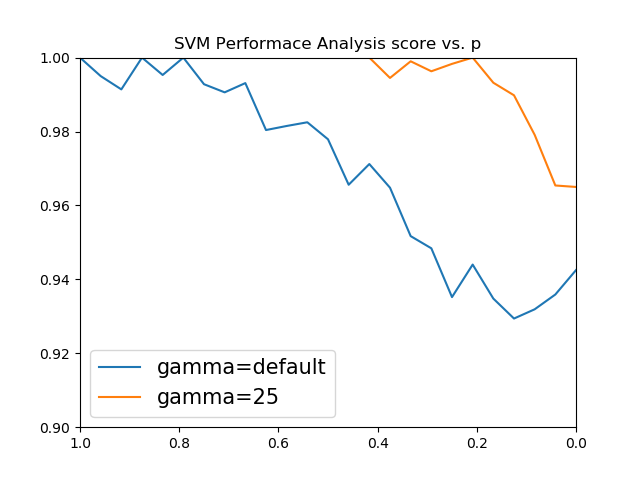
\includegraphics[scale=0.4]{svma2.png}
    \caption{rbf kernel SVM score $\gamma=$default vs. $\gamma=25$}
    \label{svma2}
\end{figure}
According to Figure.\ref{6} and Figure.\ref{7} we can see that the model will be more stable and have a better performance no matter what the value of $p$ is. 
\begin{figure}[H]
    \centering
    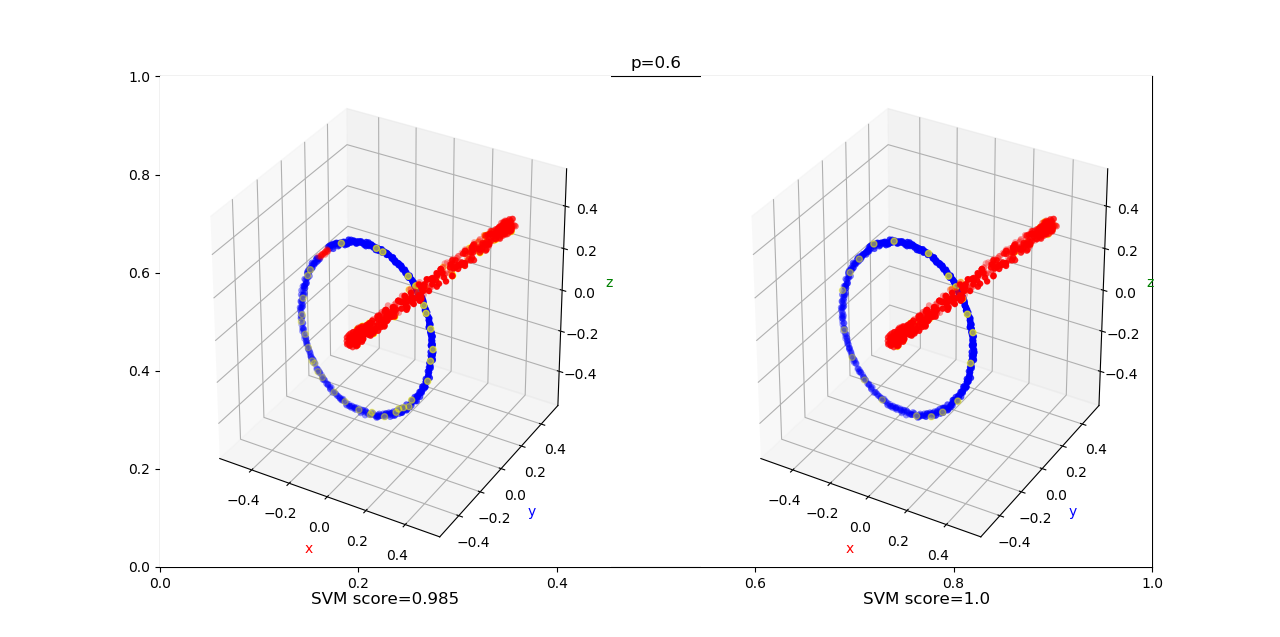
\includegraphics[scale=0.4]{8.png}
    \caption{Result when $p=0.6$ and rbf kernel with $\gamma_1=250$ and $\gamma_2=25$}
    \label{8}
\end{figure}
\begin{figure}[H]
    \centering
    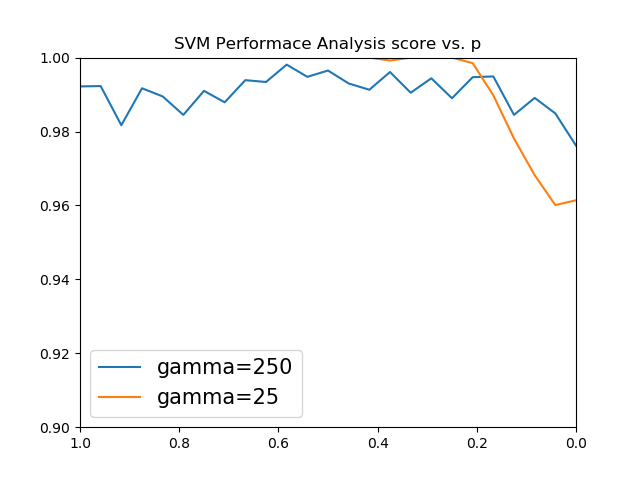
\includegraphics[scale=0.4]{svma3.png}
    \caption{rbf kernel SVM score $\gamma=25$ vs. $\gamma=250$}
    \label{svma3}
\end{figure}
However, according to Figure.\ref{8} and Figure.\ref{svma3}, if we keep increasing $p$, its performance at large $p$, which should be very simple, will become worse, it is probably because the model is overfitted. When $p\rightarrow0$ and the case become more extreme, large $p$ is a better choice since it has a more exquisite classification. In this case, my classification is based on the fact that we already know the distribution of true data, hence high $\gamma$ can lead to a good result, but it is not always the case in real practice. 
In conclusion, if we use the rbf kernel a high $\gamma$ is optimal when the data in one category are not separable but clustered in many scattered point. 
\subsection{Unsupervisied Classification PCA}
Based on previous analysis and experiment on kernel SVM, I wonder what's the performance of kernel PCA using the rbf kernel to make the data linear separable. To some extent, the kernel PCA can show the process that how SVM deal with the data, because if KPCA can make the data linear separable, SVM must can have a satisfying performance when using the same kernel. Similarly, we start with the most simple case where $p=1$.
\begin{figure}[H]
    \centering
    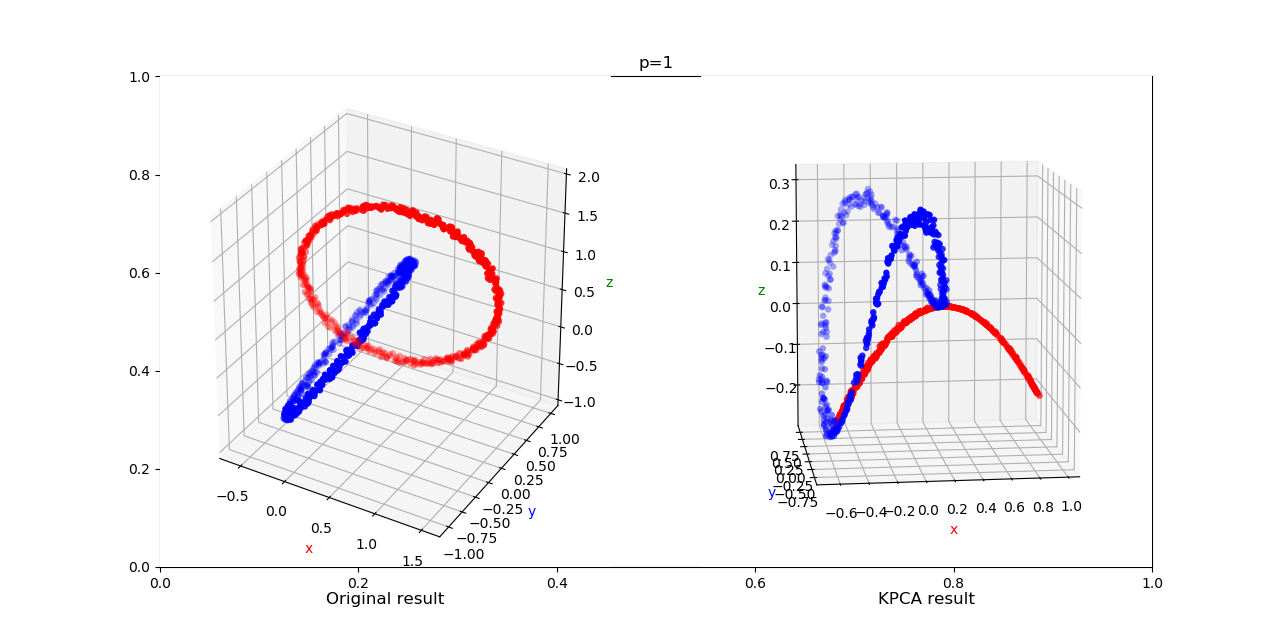
\includegraphics[scale=0.4]{PCA1.png}
    \caption{KPCA result when using poly kernel}
    \label{PCA1}
\end{figure}
When I used the polynomial kernel function, it seems that the data can't be separated linearly, this can explain why SVM has a bad classification result when using polynomial kernel. Then I switch the rbf kernel with $\gamma=$default.
\begin{figure}[H]
    \centering
    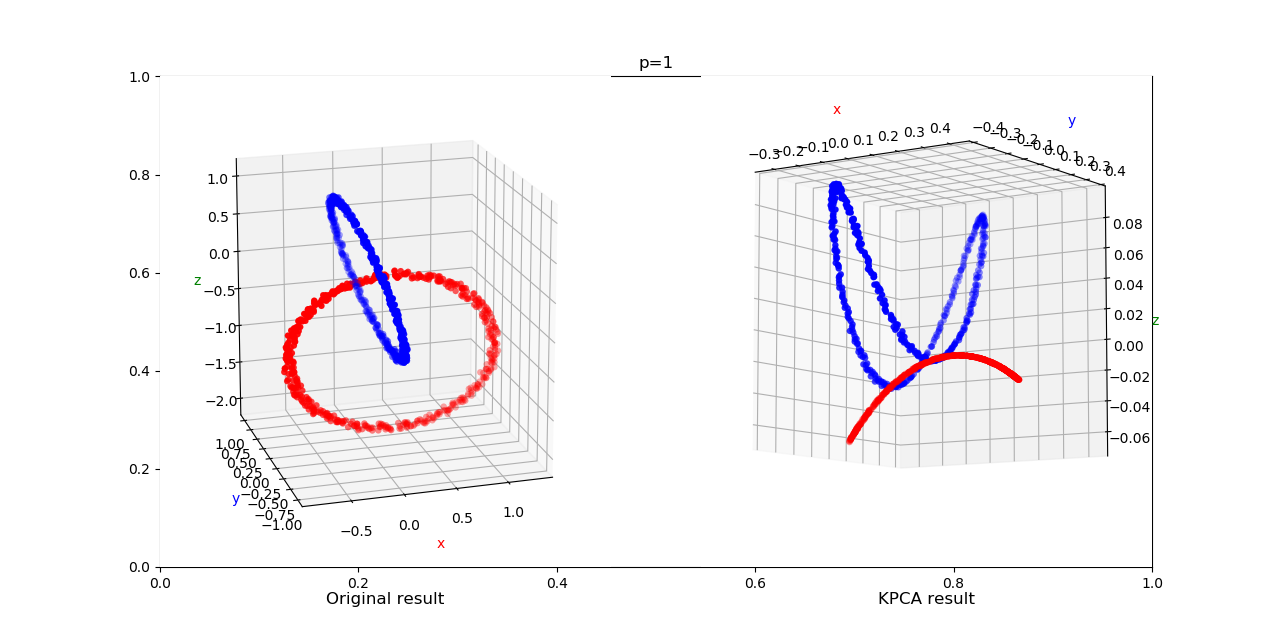
\includegraphics[scale=0.4]{PCA3.png}
    \caption{KPCA result when using poly kernel}
    \label{PCA3}
\end{figure}
Figure.\ref{PCA3} shows rbf kernel succeeds in separating the data, but it not always case, and it get worse as $p$ decreases.
\begin{figure}[H]
    \centering
    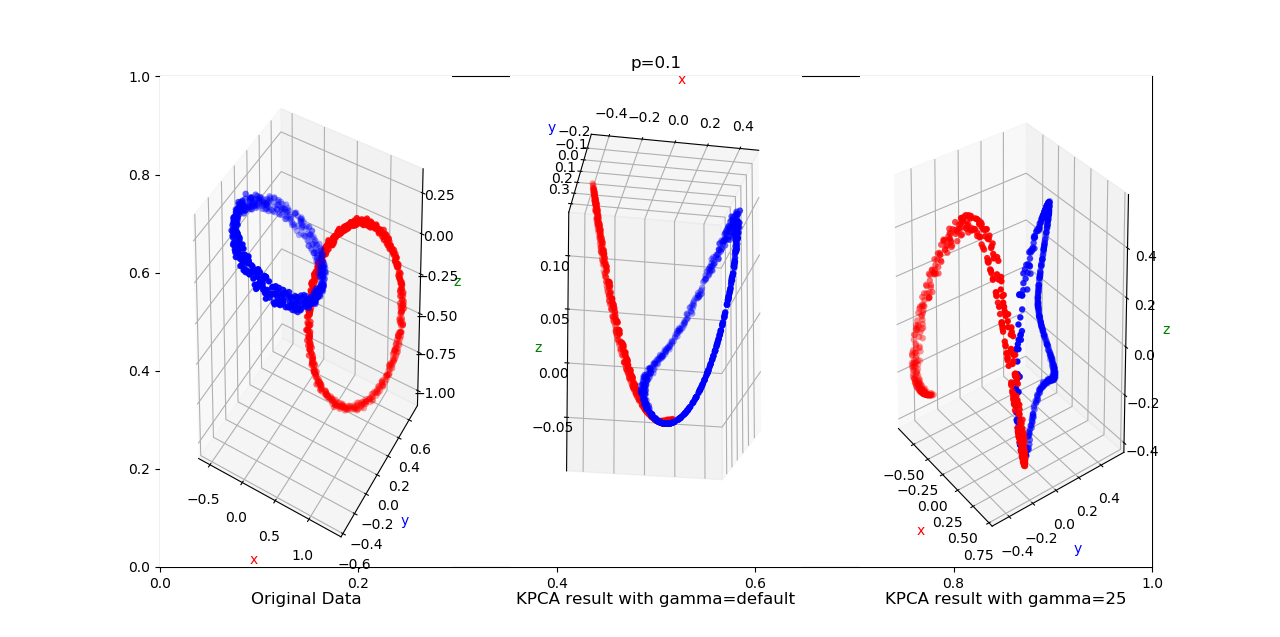
\includegraphics[scale=0.4]{PCA5.png}
    \caption{KPCA result when using different $\gamma$}
    \label{PCA5}
\end{figure}
Different from SVM cases, it seems Kernel PCA with rbf kernel can't have a significant difference when $p$ or $\gamma$ changes. That may implies that $\gamma$ only work well when we know the label of data.  
\begin{figure}[H]
    \centering
    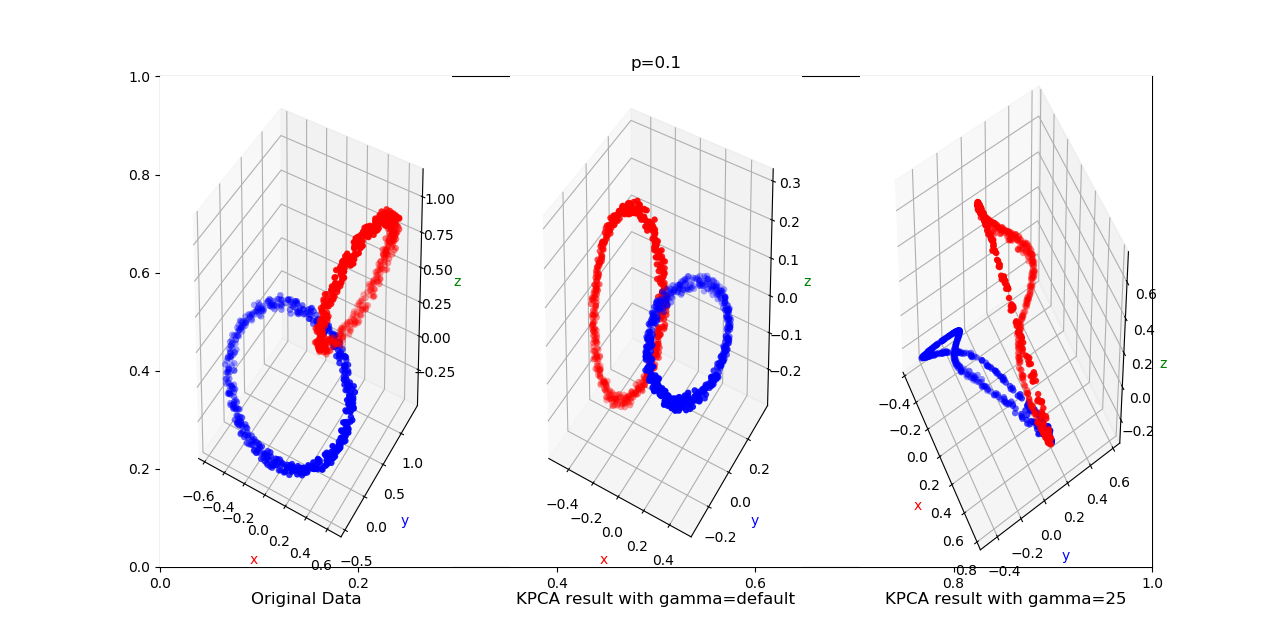
\includegraphics[scale=0.4]{PCA7.png}
    \caption{KPCA result when using different $\gamma$}
    \label{PCA7}
\end{figure}
When I put the label into the fitting process, the PCA has a similar feature like SVM with kernel rbf, where $\gamma$ seems to play a significance role in it. This proves that large $\gamma$ only works well with the label. However, for kernel PCA, we can never get the label since it's for unsupervised learning.
\section{Conclusion}
SVM is a common and quite effective classifier in practice. Compared to neuro network, the biggest feature of SVM lies is relation with the support vector, so that it can have a great performance even when we only have a few data for training. In my experiment, I only used 10\% data for training, but it still have a score higher than 90. 
\\When we're using SVM to classify data not linearly separable, the kernel's role is quite important, since it can transformed the data into a higher dimension so that it can be separated easily. It seems that rbf kernel is always the good choice because it can transform the data to infinite dimension, which means it can have the same or better performance, compared to other kernel functions, however, such feature also implies that it needs a lot of calculation. But since SVM doesn't need a lot of data, it can make up rbf's shortcoming.
\\In the process of optimization, I found the significance role of $\gamma$. The value of $\gamma$ determine the radius of each support vector in the infinite dimension, if it's larger, the radius is smaller, so we must have more support vectors for classification, hence it can increase the accuracy but also increase the risk of overfitting.
\\After playing with SVM, I apply the kernel trick into SVM and observe the role of $\gamma$, and it can't play a significance role as in the SVM. Therefore $\gamma$ seems to only be important in the supervised learning.
\begin{thebibliography}{99}
\bibitem{1}Cortes, Corinna; Vapnik, Vladimir N. (1995). "Support-vector networks" (PDF). Machine Learning. 20 (3): 273–297. CiteSeerX 10.1.1.15.9362. doi:10.1007/BF00994018.
\bibitem{2}Berwick, Robert. "An Idiot’s guide to Support vector machines (SVMs)." Retrieved on October 21 (2003): 2011.
\bibitem{3}Boser, Bernhard E.; Guyon, Isabelle M.; Vapnik, Vladimir N. (1992). "A training algorithm for optimal margin classifiers". Proceedings of the fifth annual workshop on Computational learning theory – COLT '92. p. 144. CiteSeerX 10.1.1.21.3818. doi:10.1145/130385.130401. ISBN 978-0897914970.
\bibitem{4}Hofmann, Thomas; Scholkopf, Bernhard; Smola, Alexander J. (2008). "Kernel Methods in Machine Learning"
\bibitem{5}Shalev-Shwartz, Shai; Singer, Yoram; Srebro, Nathan; Cotter, Andrew (2010-10-16). "Pegasos: primal estimated sub-gradient solver for SVM". Mathematical Programming. 127 (1): 3–30. CiteSeerX 10.1.1.161.9629. doi:10.1007/s10107-010-0420-4. ISSN 0025-5610.
\bibitem{6}Hsieh, Cho-Jui; Chang, Kai-Wei; Lin, Chih-Jen; Keerthi, S. Sathiya; Sundararajan, S. (2008-01-01). A Dual Coordinate Descent Method for Large-scale Linear SVM. Proceedings of the 25th International Conference on Machine Learning. ICML '08. New York, NY, USA: ACM. pp. 408–415. CiteSeerX 10.1.1.149.5594. doi:10.1145/1390156.1390208. ISBN 978-1-60558-205-4.
\bibitem{7}Duan, Kai-Bo; Keerthi, S. Sathiya (2005). "Which Is the Best Multiclass SVM Method? An Empirical Study". Multiple Classifier Systems. LNCS. 3541. pp. 278–285. CiteSeerX 10.1.1.110.6789. doi:10.1007/11494683\_28. ISBN 978-3-540-26306-7.
\bibitem{8}Ben-Hur, A., Horn, D., Siegelmann, H.T. and Vapnik, V., 2001. Support vector clustering. Journal of machine learning research, 2(Dec), pp.125-137.
\bibitem{9}Drucker, Harris; Burges, Christ. C.; Kaufman, Linda; Smola, Alexander J.; and Vapnik, Vladimir N. (1997); "Support Vector Regression Machines", in Advances in Neural Information Processing Systems 9, NIPS 1996, 155–161, MIT Press.
\bibitem{10}Polson, Nicholas G.; Scott, Steven L. (2011). "Data Augmentation for Support Vector Machines". Bayesian Analysis. 6 (1): 1–23. doi:10.1214/11-BA601
\bibitem{11}Platt, J., 1999. Probabilistic outputs for support vector machines and comparisons to regularized likelihood methods. Advances in large margin classifiers, 10(3), pp.61-74.
\bibitem{12}Suykens, J.A. and Vandewalle, J., 1999. Least squares support vector machine classifiers. Neural processing letters, 9(3), pp.293-300.
\end{thebibliography}
\end{document}
